\documentclass[12pt]{article}
% \usepackage[english]{babel}
% \usepackage[utf8x]{inputenc}

\usepackage{graphicx} % Required for inserting images.
\usepackage[margin=25mm]{geometry}
\parskip 4.2pt  % Sets spacing between paragraphs.
% \renewcommand{\baselinestretch}{1.5}  % Uncomment for 1.5 spacing between lines.
\parindent 8.4pt  % Sets leading space for paragraphs.
\usepackage{caption}
\usepackage{amsmath}
\usepackage{amsfonts}
\usepackage{amssymb}
\usepackage{listings}
\usepackage{siunitx}
\usepackage{verbatim}
\usepackage{hyperref} % Required for inserting clickable links.
\usepackage{natbib} % Required for APA-style citations.
\usepackage{titling}

\geometry{a4paper, margin=1in}

\begin{document}

\begin{titlepage}
    \begin{center}
        % \includegraphics[width=0.3\linewidth]{Hulogooo.png} 
        \vspace{1cm}

        \LARGE
        \textbf{RISC V Pipelined Processor}

        \vspace{1.5cm}
        \Large
        \textbf{Final Report}

        \vspace{2cm}
        \large
        \textbf{Submitted by:}\\
        Raahim Hashmi \\
        Meesum Abbas \\
        Laiba \\

        \vspace{0.5cm}
        \large
        \textbf{Research Assistant:}\\
        Maham Tabassum, Ahmed Bilal

        \vspace{0.5cm}
        \large
       \textbf{ Course Instructor:}\\
       Dr. Farhan Khan

        \vspace{1cm}
        \large
        Computer Science, Computer Engineering\\ Habib University\\
        Spring '24

        \vspace{1cm}
        \large
        Date: \today 

        \vfill
        \small
        \textit{A report submitted in fulfillment\\
        of the requirements for the lab project\\ of 
        CE/CS - 321/330: Computer Architecture}

    \end{center}
\end{titlepage}
\tableofcontents

\newpage


% \begin{abstract}
%     hello
% \end{abstract}

\section{Introduction}\label{sec:intro}
Our project involved building a 5-stage pipelined RISC V processor capable of executing a bubble sorting algorithm. We completed the following tasks:

\begin{enumerate}
    \item Converted the bubble sort code in python to RISC V assembly code and verified it on the Venus simulator. (Then converted the 32 lw and sw to ld and sd and other changes that were required to shift from 4-bytes to 8-bytes). Modified the lab 11 single-cycle processor to run the bubble sort code.
    \item Pipelined the processor and tested individual instructions to ensure the pipelined version worked correctly.
    \item Implemented hazard detection circuitry to identify and handle hazards (data, control, and structural) by using techniques such as forwarding, stalling, and flushing the pipeline.
    \item Compared the performance of running the array sorting program on a Single Cycle Processor with a pipelined RISC-V Processor in terms of execution time.
    
\end{enumerate}

\section{Task 1}\label{task1}
    \subsection{Bubble Sort Pseudocode to Machine Code}\label{task1-0}
        We first implemented the sorting algorithm in RISC V assembly on the Venus simulator, which we had done in a previous Lab. Then we modified it to support double word storing, loading from the data memory. We then converted the assembly code to machine code and initialized the instruction memory with the machine code. And finally, then ran the code on the single-cycle processor to sort an array of numbers. The following is the assembly code for the bubble sort algorithm:
        
        \begin{figure}[htbp!]
        % \begin{center}
            \centering
            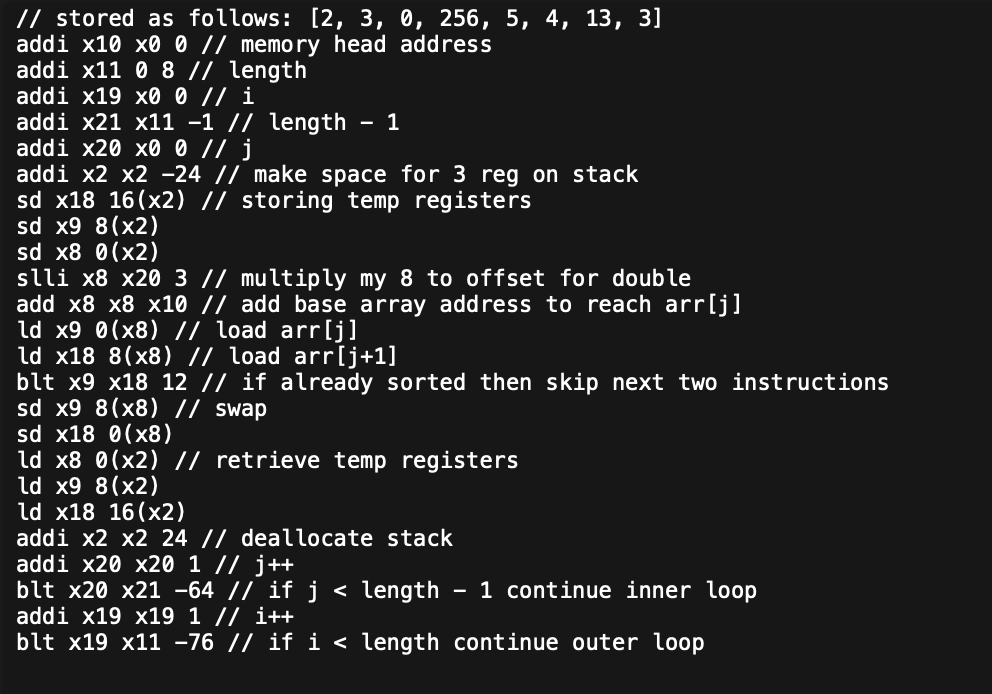
\includegraphics[scale = 0.7]{images/bubbleSort.png}
            \caption{Assembly code for bubble sort}
        % \end{center}
        \end{figure}
        \begin{figure}[htbp!]
        % \begin{center}
            \centering
            % \includegraphics[scale = 0.7]{registers2.png}
            % \caption{Initializing instruction memory with machine code}
        % \end{center}
        \end{figure}
        
\newpage

    \subsection{Bubble Sort Implementation Single Cycle}\label{task1-1}
        We made some minor modifications to the lab 11 module where we instantiated all modules together to make the processor. We also modified ALU and instruction memory code and added a branch unit code to support branch operations. In ALU code, we added functionality for funct3 bit of blt, and also changed the 4-byte offset to an 8-byte offset as we have a 64-bit processor. We also added functionality for slli. We then initialized the instruction memory with the machine code and ran the code on the single-cycle processor to sort an array of numbers. The following is the manually written machine code in verilog:
        % \end{lstlisting}

\subsection{Simulation Output}\label{code1}
    \begin{figure}[htbp!]
    % \begin{center}
        \centering
        % \includegraphics[scale = 0.53]{task1 sim.jpg}
        \caption{Snippet of simulation output}
    % \end{center}
    \end{figure}
   
    \begin{figure}[htbp!]
    \begin{center}
            
            % \includegraphics[scale = 0.6]{task1 sorted.jpg}
            \caption{Sorted array}
    \end{center}
    \end{figure}

\section{Task 2}\label{task2}
    \subsection{Pipelined RISC V Processor}\label{task2intro}
    After implementing the algorithm on the single-cycle processor we next modified the code to pipeline the modules. For that, we referred to Dr. Farhan's lecture slides and then added the following modules to act as intermediate registers for the pipeline:
    \begin{itemize}
        \item IF/ID
        \item ID/EX
        \item EX/MEM
        \item MEM/WB
    \end{itemize}
    These registers help store the value of previous instruction's data and pass it along the pipeline. We tested each instruction separately to make sure that the pipeline was working correctly. We also implemented the forwarding unit by modifying the previous code so that we can forward data in the pipeline. The forwarding unit will be integrated with the hazard detection unit which determines where to forward data.
\newpage

\subsection{Simulation Output}\label{code2}
    \begin{figure}[htbp!]
    % \begin{center}
        \centering
        % \includegraphics[scale = 0.31]{task2.jpg}
        \caption{Snippet of simulation output}
    % \end{center}
    \end{figure}

\section{Task 3}\label{task3}
\subsection{Detecting Hazards and Resolving them}\label{hazards}
   Data and Control hazards are dealt with within the code by implementing hazard detection circuitry and stalling/flushing the pipeline when needed. These hazards mostly arise from dependencies in the code or if the data needs to be forwarded further at some point. For this, we tried to implement the hazard detection unit that controls when to stall the pipeline or forward the data by signaling the forwarding unit to stall or flush the pipeline.

\newpage
\subsection{Simulation Output}\label{code3}

    \begin{figure}[htbp!]
    % \begin{center}
        \centering
        % \includegraphics[scale = 0.4]{task32.jpg}
        \caption{Snippet of simulation output}
    % \end{center}
    \end{figure}
    \begin{figure}[htbp!]
    % \begin{center}
        \centering
        % \includegraphics[scale = 0.31]{task3.jpg}
        \caption{sorted array}
    % \end{center}
    \end{figure}

\section{Performance Comparison}\label{performance}
    Pipelined processors are usually faster than non-pipelined processors, but in our case, the pipelined processor is not functioning optimally, with a latency of about 6000ns, which is longer than the 3000ns latency of the non-pipelined processor. Despite the fact that we were able to implement the pipelining of the processor, it came with many issues in efficiency. To improve the performance of our pipelined processor, we need to analyze and optimize its design.

\section{Conclusion and Challenges}\label{performance}
    It was challenge for us to coordinate with each other and specify a time to work on together, so we had to divide the work. That too, however, came with challenges cause one of us (Meesum) works on a mac which does not support vivado. He had to use VS Code, which was still challenging as there was no way of getting the schema of the code. However, we used github and worked as a team to overcome the issues, while dividing the tasks as well. We were able to implement the pipelined processor and the hazard detection unit, and it is working perfectly as 5-cycle pipelined processor. The performance ... 

\section{References}

[1] Book. \textit{Course Book}. Computer Organization and Design: The Hardware/Software Interface RISC-V Edition by David A. Patterson, John L. Hennessy
[2] Lecture Notes. \textit{Dr. Farhan Khan}. Computer Architecture, Habib University

\section{Appendix}
The GitHub link for our project can be found \href{https://github.com/RaahimHash/Pipelined-RISC-V-Processor}{here}.

    
\end{document}